\chapter{Background and Related Word}
\label{chptr:concepts}

%In this chapter, an overview about popular patterns and characteristics for building safe and reliable systems, as well as about \gls*{DDS}, is presented.
%Afterwards, mathematical concepts for evaluating the safety and reliability of a system, are pointed out.
%At first, however, a selection of related work that uses \gls{DDS} in safety critical applications, is presented.

\section{Data Distribution Service}
\Gls*{DDS} is a \gls*{DCPS} model for machine-to-machine communication, that is specified by the \gls*{OMG}~\cite{omgDDSspec}.
It is specified that the model should, for practical use, be implemented as a middleware, to directly interface with the underlaying \gls*{OS}.
The model follows the concept of a global data space to facilitate data exchange among entities based on type and content.
Central entities in the design are \texttt{Publishers} and \texttt{Subscribers}, while data exchange is based on \texttt{Topics}.
A Publisher is used for sending data of different types.
In order to send specifically typed data, a \texttt{DataWriter} object is used, which acts as a typed interface to a Publisher.
On the other side, a Subscriber is used to receive data and make it accessible to the receiving application.
The equivalent of the DataWriter for the Subscriber is the \texttt{DataReader} object.
A Topic acts as the connecting element between publishing entities on the one side and subscribing entities on the other.
Any forecasting of when and how data is published to a Topic or received by a Subscriber is made possible through so called \glspl*{QOS} policies.

The usefulness of \glspl*{DDS} for containerization technologies in automotive architectures has been studied by Kugele et. al~\cite{KugeleDataCentricForAuto}.
Although their findings are based on containerization technologies and therefore not very resilient for this work, Kugele et. al showed that the applicability of \gls*{DDS} with regards to safety, certification and security depends on the actual implementation's characteristics~\cite{KugeleDataCentricForAuto}.
Therefore, Vortex OpenSplice DDS is used thoughout this thesis.
Vortex OpenSplice DDS is developed and maintained by ADLINK and has been proven in practice to meets the requirements towards safety, certificability and security, demanded by~\cite{KugeleDataCentricForAuto}.

\section{Techniques for Safety and Reliability Evaluation}
Reliability is, by IEEE 610.12-1990, defined as the ability of a system or component to perform its required function under stated conditions for a specified period of time~\cite{ieee610.12}.
The definition of reliability used in this work is the following:

\begin{definition}
Reliability is a system's ability to not have any failure for a specific period of time.
\end{definition}

This definition, however, assumes the definition of a failure, which is deduced from the IEEE reliability definition as follows:

\begin{definition}
A failure of a system or a system component is an incorrect behaviour of this system or this system component that lets it not perform its required function.
\end{definition}

Mathematically, reliability can be defined as a function of time which expresses the probability that a system is operating as specified at a time $t_1$, given that it was operating as specified at time $t | t \leq t_1$.
A system is said to be safe, when its number of failures is small~\cite{HollnagelSafety}.
In other words, safety is defined as a system's probability to not have any failures that would lead to a serious outcome in a specified time span~\cite{GeffroyMotetDependableComputing}.
The serious outcome depends on the execution environment and is often linked to a catastrophic failure.

Based on these definitions, it can be conducted that the reliability of a system can only be finally assessed when the system's environment, the reliability of the system's components and the operations performed by the system are known.
Futher, in order to specifically evaluate a system's safety, possible sources of failures and their consequences need to be known.
In order to be able to evaluate and compare different architectural pattern towards their safety characteristics, the definition of \texttt{intrinsic safety}, made by~\cite{BoulangerStandards}, is used in this work.

\begin{definition}
A system is said to be intrinsically safe if one can be certain that any failure of one or more components of that system will only result in its becoming more permissive.
In the railway context, a complete stoppage is generally the safest state.
\label{def:intrinsic_safety}
\end{definition}

In other words, an intrinsically safe system can fail, as long as it stops the train when doing so.
In order for the system to be able to stop the train in case of an intrinsic failure, the system needs to be able to detect any intrinsic failure.
It follows from~\autoref{def:intrinsic_safety}, that for safety-critical systems, the system's reliability is completely included in the system's intrinsic safety~\cite{BoulangerStandards}.
This allows to analyze a systems safety and reliability by only considering the system's architecture and components and independently of its environment and applied computations.
Thus, for the rest of this thesis, only the system's intrinsic safety will be evaluated and the term safety will be used synonymously for intrinsic safety.
\begin{definition}
A system, in the course of this thesis, is said to be safe when it reliably detects intrinsic failures and stops the train in the presence of an intrinsic failure.
\label{def:safety}
\end{definition}

For the rest of this thesis, in order to describe the consequences of failures, the terms \texttt{error} and \texttt{fault}, from the context of testing, are used~\cite{AmmannOffutt2016}.

\begin{definition}
A fault describes a static defect of a system.
\end{definition}

\begin{definition}
An error marks an incorrect internal system state that is the manifestation of some fault.
\end{definition}

\subsection{Safety Evaluation}
A required condition for a system to be safe is that the system is reliable~\autoref{def:safety}.
One method of analyzing a system's reliability is through mathematical functions of time, for example the \texttt{exponential failure law}~\cite{GeffroyMotetDependableComputing}.
It describes a component's reliability as an exponential function on time.
\begin{equation}
R(t) = e^{-\lambda t}.
\label{eq:expFailureLaw}
\end{equation}
The parameter $\lambda$ encodes the probability of failures occuring in a certain time span, typically in an hour.


\todo{Describe techniques used in following safety evaluation/analysis}

\section{Redundancy Patterns}
A typically applied technique for handling and masking failures in a system is redundancy~\cite{TanenbaumSteen07}.
Failure masking is the concept of catching the effects of internal system failures, so that they do not effect the system's environment.
For redundancy, additional resources are added to a system, that would not be required when no internal system failures ever happen.
Barry Johnson defines redundancy in the following way~\cite{BarryFaultToleranceAnalysis}:
\begin{definition}
The concept of redundancy implies the addition of information, resources, or time beyound what is needed for normal system operation.
Redundancy can take one of several forms, including hardware, software, information, and time redundancy.
\end{definition}

Each form of redundancy has its unique characteristics and patterns, which are presented in the following.

\subsection{Hardware Redundancy}
In hardware redundancy, additional replications of physical components are added to the system.
This typically increases the system's safety by masking internal failures, but also increases the system's cost.
In general, a system's safety can be improved when using components that are based on different internal components.
Using different components in redundancy patterns is called diverse redundancy, while replicating the same components is called homogeneous redundancy\todo{Ref}.
Using diverse redundancy has the benefit that it reduced the effect that common core errors have on a system's or component's safety.

Johnson subdevides hardware redundancy into two parts, namely passive and active redundancy.
In passive hardware redundancy, a voter or consensus algorithm is used to reduce a number of redundant outputs to a single output, in order to prevent individual internal failures from propergating out of the system.
In active hardware redundancy, the system tries to detect and repair any internal failure.
While \gls*{MOON} systems are a typical example of passive hardware redundancy, standby redundancy is often used as an example of active hardware redundancy.

\paragraph{M-out-of-N Redundancy}
\begin{figure}[!hb]
	\centering
	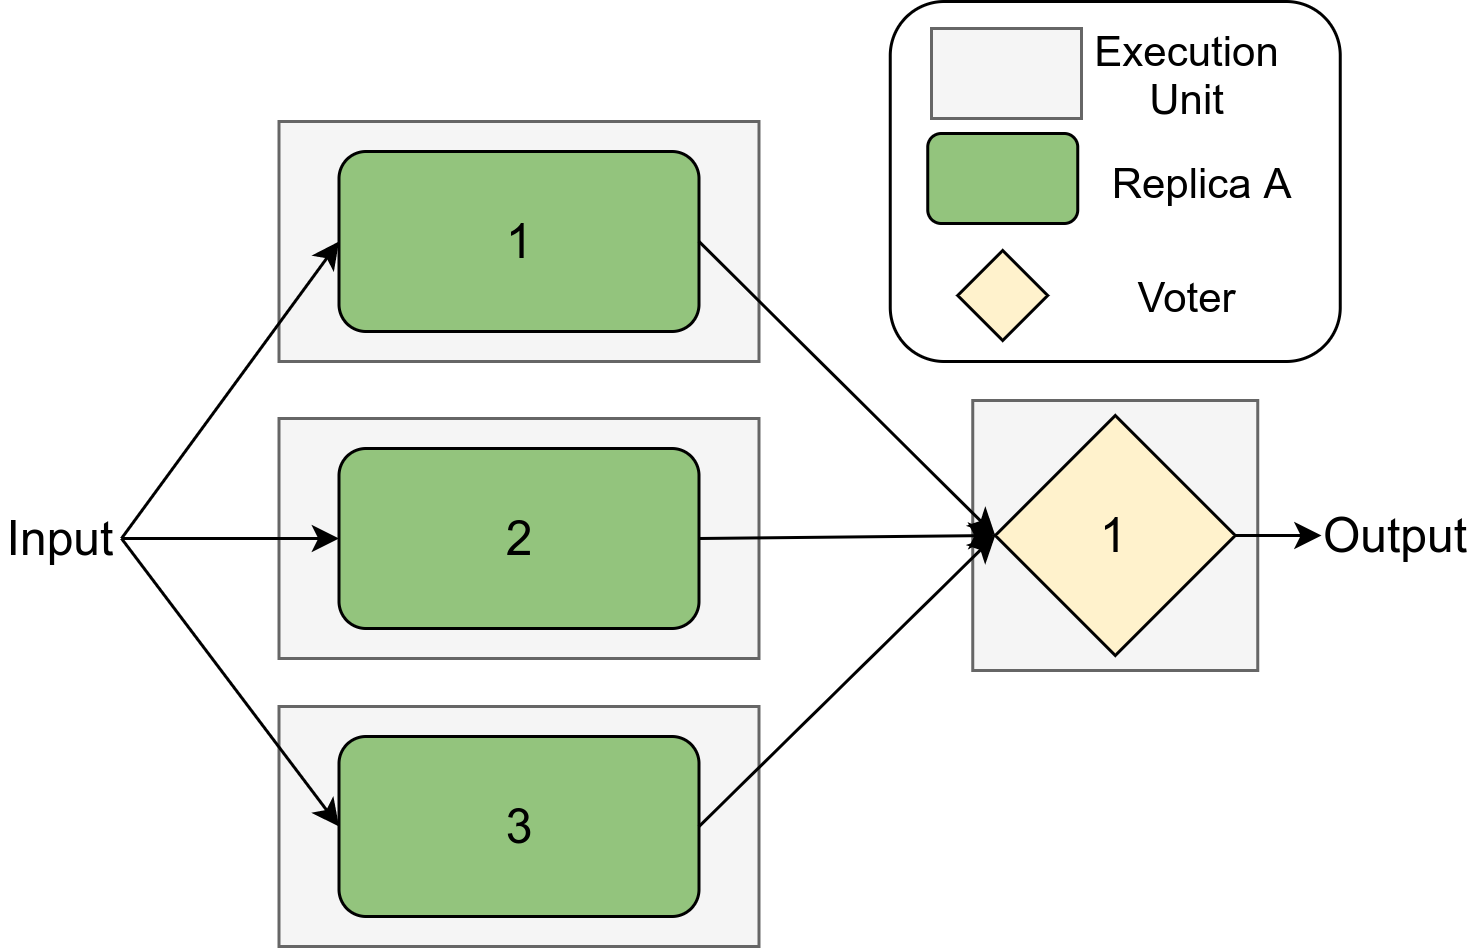
\includegraphics[width=0.75\linewidth]{images/Classical2OO3}
	\caption{Classical 3-out-of-2 redundancy, also known as \Gls*{TMR}.}
	\label{fig:Classical2OO3}
\end{figure}

One of the most common versions of \gls*{MOON} systems is \gls*{TMR}~\autoref{fig:Classical2OO3}.
In \gls*{TMR}, three replicas are receiving the same input and performing the same work in parallel.
A voter collects the individual outputs and reduces them to a single system output based on a majority vote.
The system output must qualify the characteristic that at least two out of the three replicas agree on this output.
This allows the entire system to still produce a correct output even in the presents of a faulty replica.
All replicas, as well as the voter, are running on individual hardware units.

The weakness of \gls*{TMR} is the voter, because it marks a single point of failure.
Therefore, the voter's reliability in this system has to be very high compared to the three replicas, because the entire system's dependability cannot be higher than the voter's dependability.
As an alternative to the voter, a consensus algorithm could be used.
A consensus algorithm is applied to let all components in the system agree on a single output value.
This single output value is required to be proposed by at least one component~\cite{lamport2001paxos}.
While not having a single point of failure anymore, consensus approaches typically introduce a communication overhead and lead to rigid configurations~\cite{GamerIncreasingMOON}.

\begin{figure}[!hb]
	\centering
	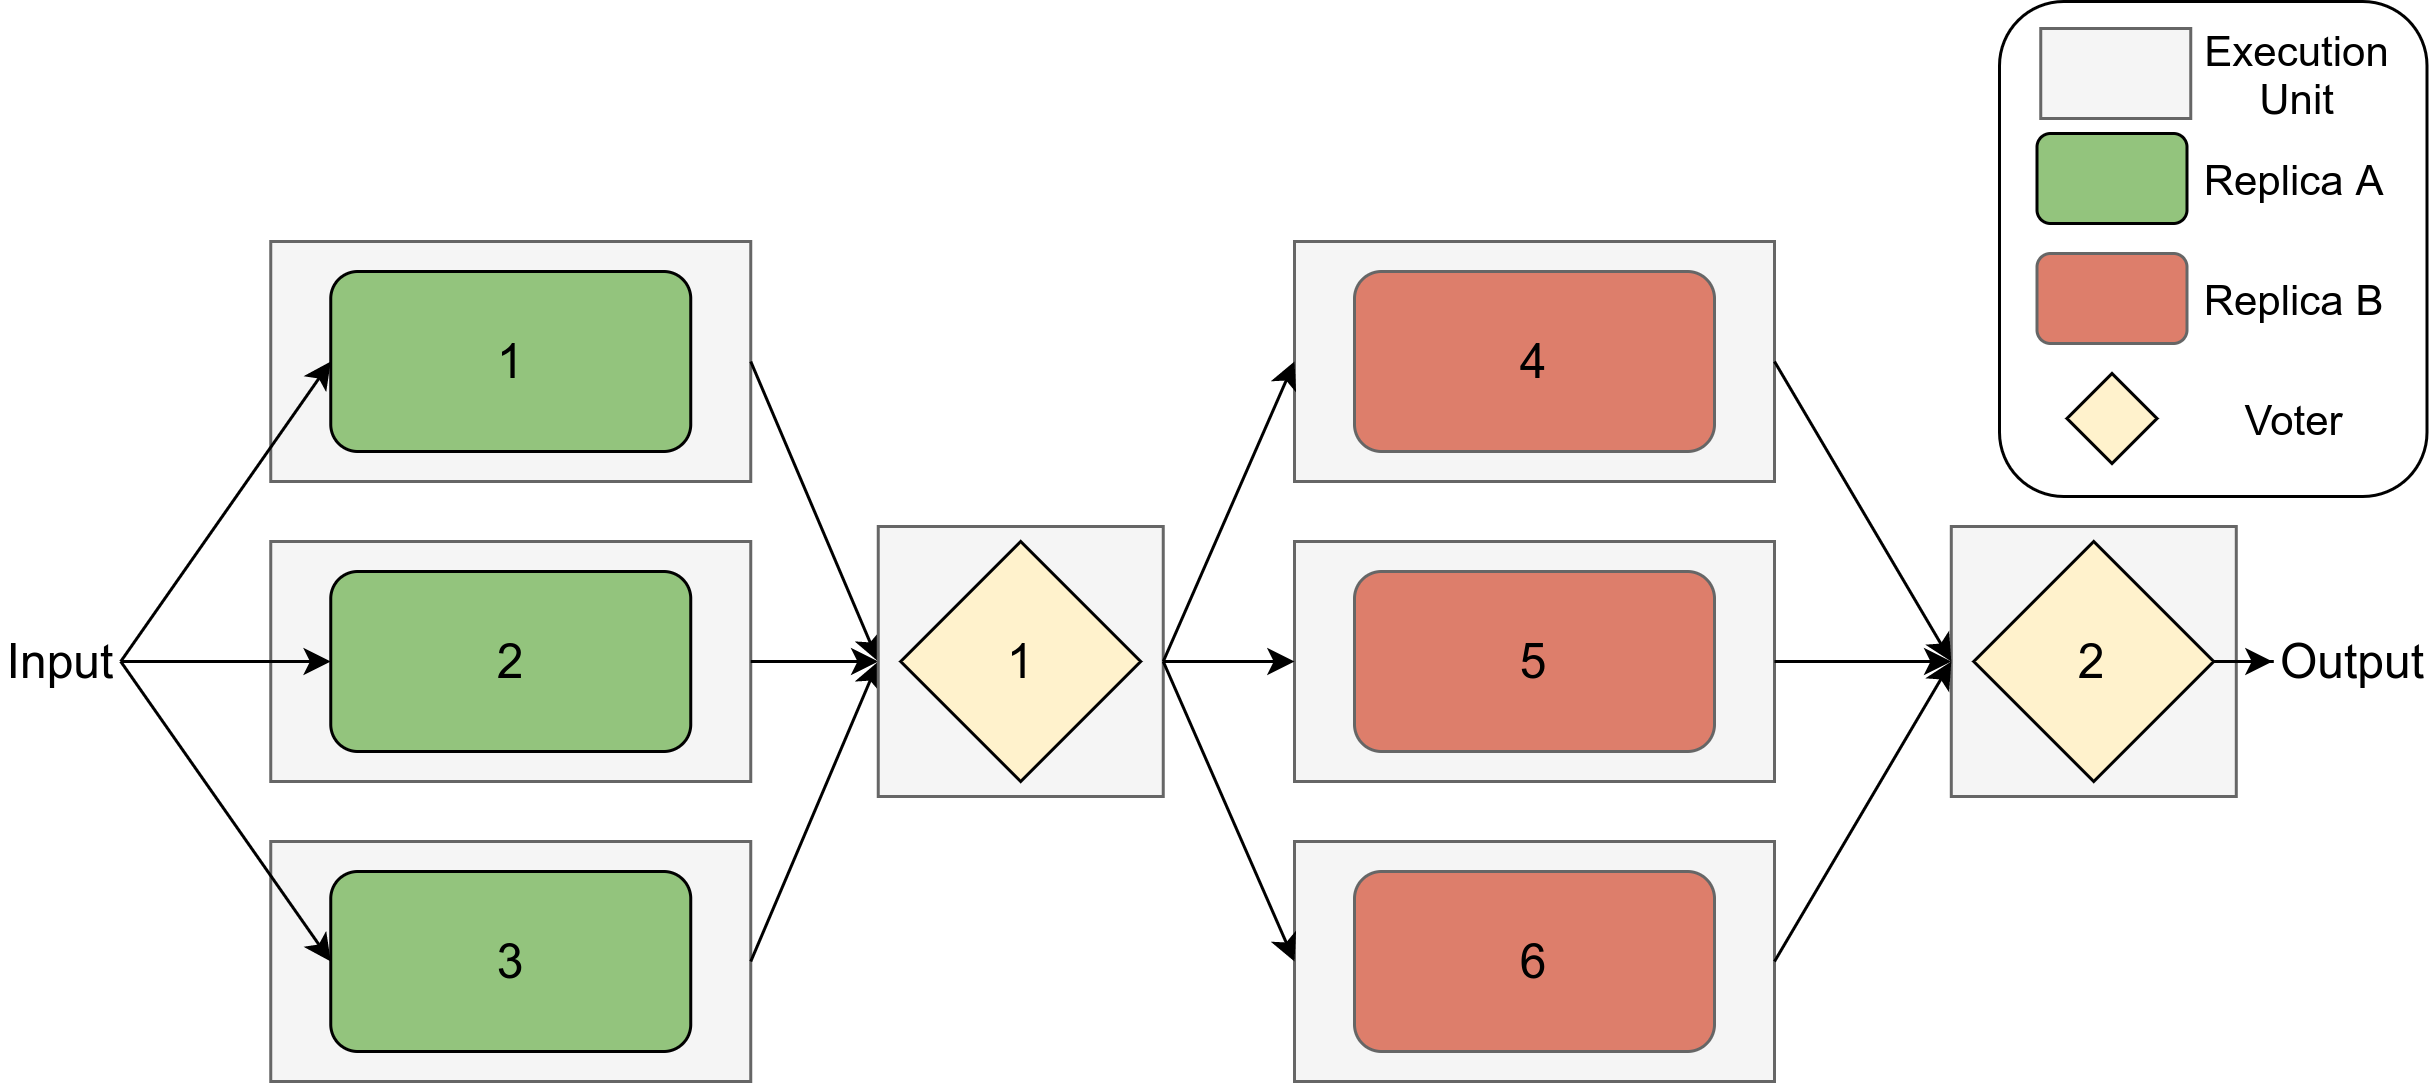
\includegraphics[width=0.75\linewidth]{images/IntermediateVoting}
	\caption{Intermediate voting could be applied to reduce the effect of partial results on the final output.}
	\label{fig:IntermediateVoting}
\end{figure}

Instead of having one voting about the final result, the calculations could be modularized and votings on intermediate results could be made.
This would have the benefit of masking intermediate faults and not letting them influence further calculations.
An example of how this could be achieved is depicted in~\autoref{fig:IntermediateVoting}.

\paragraph{Standby Redundancy}
\begin{figure}[!hb]
	\centering
	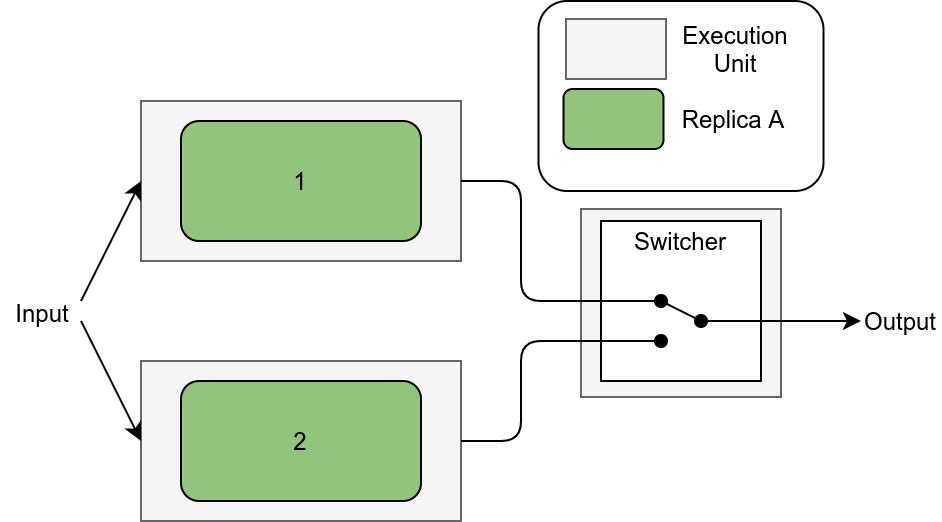
\includegraphics[width=0.75\linewidth]{images/ActiveSelectionRedundancy}
	\caption{With standby redundancy, a system can recover from individual component errors by replacing faulty components.}
	\label{fig:StandbyRedundancy}
\end{figure}

As stated above, standby redundancy is an example of active hardware redundancy and build on the concept of error detection, location and recovery.
In an exemplary case of an internal component failure, the resulting error needs to be detected and the faulty component needs to be located, so that the system can recover from the error by replacing the faulty component by an identical spare component.
An example is depicted in~\autoref{fig:StandbyRedundancy}, where two identical replicas are used, one as a primary and one as a secondary component.
A switching element observes the active component and, when no internal failure in the active component happened, leads the active components output out of the system.
As soon as the switching element detects an internal failure, it excludes the active component from the system and takes the secondary component's output as the system's output, which thereby becomes the active component.
When the secondary component is already running when the switching happens, this is called hot standby redundancy.
When the secondary component needs to be turned on before it can be used as the active component, this is called cold standby redundancy.

\subsection{Software Redundancy}
One speaks of software redundancy, when redundancy concepts for error detection are implemented in software.
Examples for software redundancy are heartbeat messages to validate a component's accessibility, component-checking or software voters.
In component-checking, a program is used to monitor and validate a component's hardware, for example its memory, clock or \gls*{CPU}.
Thereby, it can be qualified whether a specific component's output can be considered valid or not.
This state is summarized into the term \texttt{internal consistency}.

\begin{definition}
A system or a component is said to be internally consistent, when any failure of this component is not based on a fault of its internal hardware.
A system's or component's internal consitency can be determined by component checking mechanisms.
\end{definition}

Further, voting or consensus algorithms can be implemented in software.
Similar to homogeneous and diverse hardware redundancy, diverse implementations of the same software can be used to reduce the effect of faults in a software.

\subsection{Information and Time Redundancy}
The addition, adding redundant information can allow the detection, masking and recovery from faults~\cite{BarryFaultToleranceAnalysis}.
Examples for information redundancy include Hamming codes~\cite{HammingCodes}, checksums or information duplication.
All information redundancy concepts share that they somehow encode redundancy into some information that can later be decoded.

\begin{figure}[!hb]
	\centering
	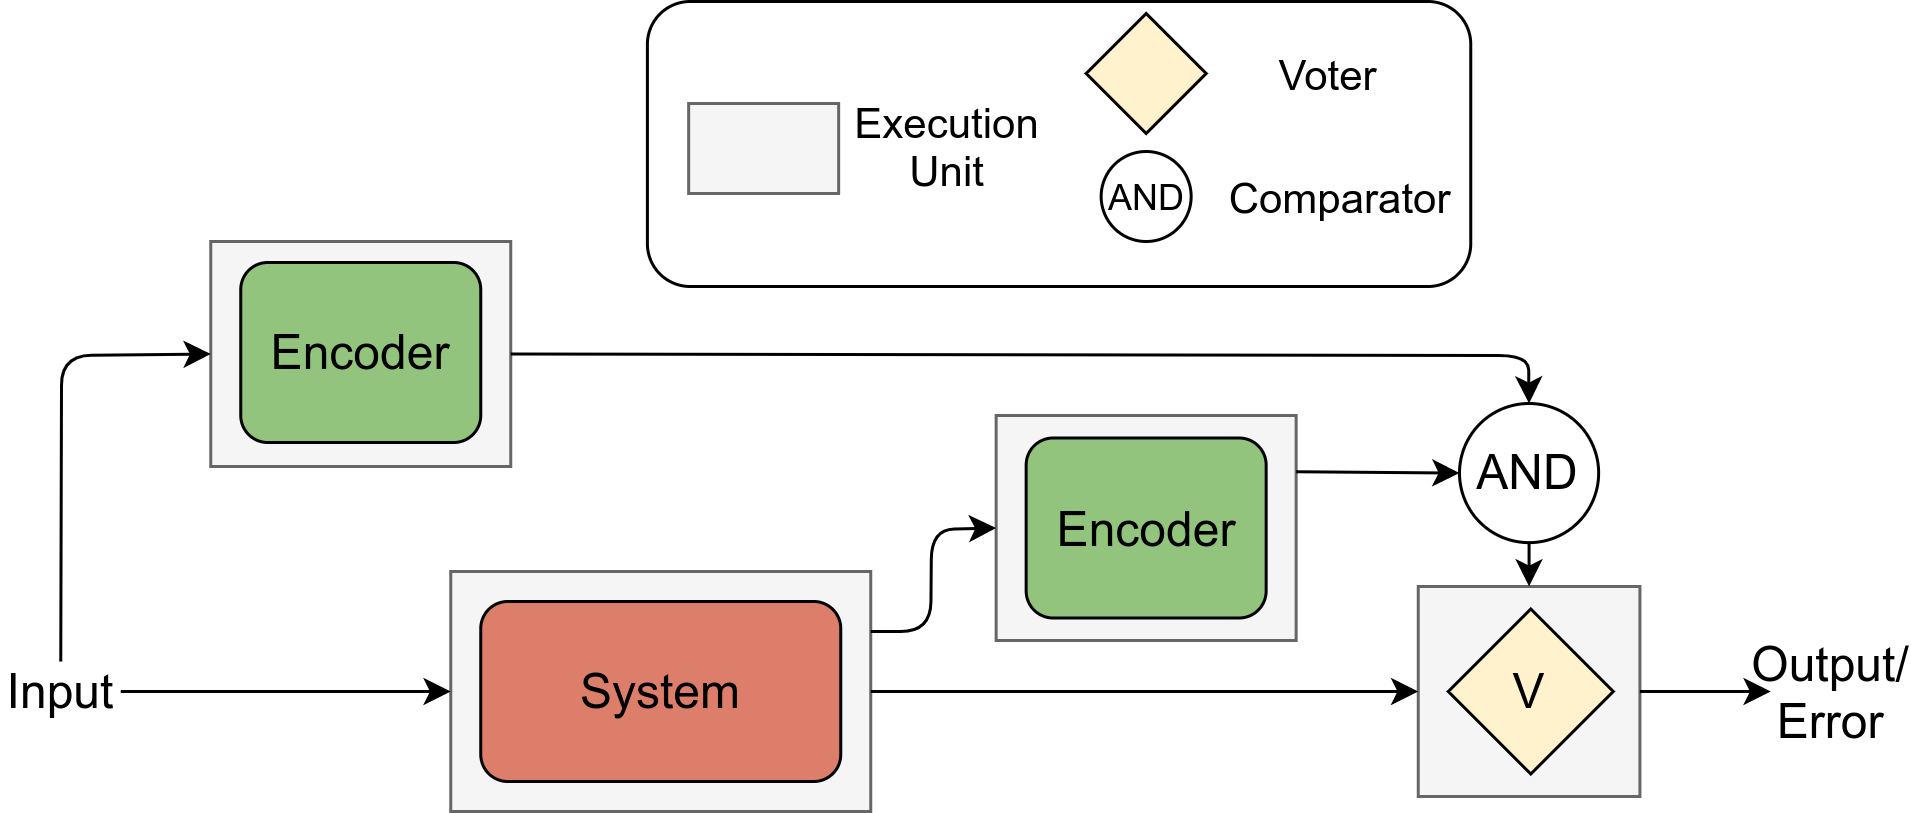
\includegraphics[width=0.75\linewidth]{images/ECC}
	\caption{Using information redundancy and error checking methods, error detection can be achieved~\cite{Su2005ECC}.}
	\label{fig:ECC}
\end{figure}

Another way of adding redundancy is to perform the same operation multiple times at different points in time.
This concept is called \texttt{Time Redundancy} and has the benefit that it does not require many additional physical components.
Thereby, permanent faults in a system can be detected.

\autoref{fig:ECC} depicts an example of a combination of information and time redundancy using \gls*{ECC} techniques.
Therefore, an encoder encodes potential outputs for certain inputs and transmits this redundant information together with the input data.
After the system produces an output based on its input information, another encoder encodes the output, which is afterwards compared to the encoded input.
When there are anomalies between the system's input and its output, safety operations can be initiated.
The encoding function must be choosen so that it allows the detection of faults in the system, such as arithmetic shifting.

\section{Related Work}

Alapan Chakroborty demonstrates a development process of a reliable, safe and fault-tolerant system using redundancy methods by an example of railway signalling~\cite{ChakrabortyFaultTolerantRailway}.
He argues that every fault tolerant system needs to build upon real-time software solutions.
This requires both logical, as well as timing correctness which can only be achieved by correct redundancy management such as fault-propagation, synchronization and consensus among replicas.
At a fail-safe design's heart lies fault idenfication, masking and recovery.
Therefore, in a first step, each redundant design should be subdevided into redundant elements that are not affected by any fault from outside the element.
Chakroborty calls these redundant elements \glspl*{FCR}.
As a second step, he proposes to define interface between the \glspl*{FCR} so that they do not interfere with each other.
These two steps form a necessary precondition to be able to predict the probability of failures in the system.

In order for the system to reduce redundant results to a single result and to mask failures, the concept of voting is demanded.
Voting, as Chakraborty claims, requires the \glspl*{FCR} to be in identical states, to provide all redundant hardware with the same input and to ensure a real-time concurrent operation of the same computations on each \gls*{FCR} for synchronization.
Finally in the work, the shown method is performed on developing a railway signalling system.

An overview about possible redundancy concepts for the railway domain is provided by Bemment et. al~\cite{BemmentEvaluationOfRedundancy}.
They further made a cost, benefit and performance analysis for each presented concept.


In this work, the concepts proposed by Bemment et. al are extended based on the steps by Chakraborty and by using and evaluating the feasibility of \gls*{DDS} for redundancy in the railway context.
The redundancy evaluation is made based on a simplified example, because Bemment et. al pointed out that an in depth redundancy evaluation can only be made for well defined use cases where hazards, risks and potential accidents are known.
An overview about about possible accidents in railway is given by~\cite{ERTMSRailwayAccidents}.
\\

The CENELEC 50128 standard is a norm for software creating processes for railway applications, so that the build software can be considered safe.
The 2011 version of CENELEC 50128, as well as resources needed to achieve a set level of assurance, are presented by Jean-Louis Boulanger~\cite{BoulangerStandards}.
Describing a CENELEC 50128 design process for each software artefact described and used in this thesis is outside its scope.
However, each software indended to be used in railway practice should pass the CENELEC 50128 norm.
\\

The \gls*{DDS} is already successfully deployed in distributed time- and safety critical environments.
One example is given by Bijlsma et. al~\cite{DistributedSafety2020}, who extended the E-Gas layered monitoring concept to handle faults in a distributed and redundant system.
\Gls*{DDS} is applied to facilitate a reliable communication among individual components in the system.
An other example is given by Hadiwardoyo and Gao, who proposed the use of \gls*{DDS} in security cameras for subways using \glspl*{QOS}~\cite{DDSInSubways}.
A more general approach of how \gls*{DDS} can be used for enabling communication in distributed as well as time- and safety-critical environments, is given by García-Valls et. al~\cite{GarciaVallsDDSInDistributed}.
They used a simple design of sensor data reading and monitoring to benchmarked the middleware's communication performance with different \glspl*{QOS}.
Their results show that the communication performance remains stable even under heavy load.

Even though they applied a different \gls*{DDS} implementation than in this work, the network topologie and used hardware are comparable, which renders the results from García-Valls et. al useful for this work.











































\iffalse

Dependability is a characteristic for computing systems to ''deliver [a] services that can justifiably be trusted''~\cite{AvizienisDependability2001}.


\subsection{Reliability Models}
Geffroy an Motet present two reliability models, namely the exponential law and the Weinbull law, but argue that the exponential law is most commonly used for electronic systems~\cite{GeffroyMotetDependableComputing}.

The exponential law describes a component's reliability as an exponential function.
\begin{equation}
R(t) = e^{-\lambda t}.
\label{eq:expFailureLaw}
\end{equation}
As described above, a system's reliability by definition decreases over time, which is expressed in~\autoref{eq:expFailureLaw}.
The parameter $\lambda$ encodes the probability of failures occuring in a certain time span.
During this work, the value for $\lambda$ is considered to be constant, although in practice it would change over time following a \texttt{bathtub courve}~\cite{GeffroyMotetDependableComputing}.

In order to make use of the exponential failure law, Berry W. Johnson proposes two analytical techniques for analyzing a system's reliability, namely combinatorial modeling and Markov modeling~\cite{BarryFaultToleranceAnalysis}.
He argues that, while in serial systems each element needs to operate in the prescribed way for the system to be reliable, in parallel systems only a subset of all components needs to function correctly.

\paragraph{Serial System}
A serial system is a system that contains no redundancy~\cite{BarryFaultToleranceAnalysis}.
Thus, the reliability of a serial system is directly dependent on the propability that all individual components work correctly.
%Therefore, the reliability of a serial system, consisting of $N$ individual components, at time $t$ can be calculated as
%\begin{equation}
%R_s(t) = P\{ R_1(t) \cap R_2(t) \cap \dots \cap R_N(t) \}
%\end{equation}
%where $R_s(t)$ describes the reliability of the entire serial system at time $t$ and $R_i(t)$  being the probability of component $C_i$ working correctly at time $t$.
For independent components, which follow the exponential failure law, holds~\cite{BarryFaultToleranceAnalysis}:
\begin{equation}
R_s(t) = e^{\sum_{i = 1}^N \lambda_i t}
\label{eq:combReliabSerial}
\end{equation}

\paragraph{Parallel System}
In a parallel system, as defined by Johnson, where $N$ identical components are working in parallel, only one individual component is required to work correctly for the entire system to work correctly.
A parallel system's reliability is therefore reciprocal to the probability of all $N$ components failing at the same time.
%
%This is expressed through
%\begin{equation}
%R_p(t) = P\{ R_1(t) \cup R_2(t) \cup \dots \cup R_n(t) \}
%\end{equation}
%where $R_p(t)$ being the reliability of the entire parallel system at time $t$ and $R_i(t)$ being the probability of component $C_i$ working correctly at time $t$.
When all $C_i(t)$ are independent and follow the exponential law, a parallel system's reliability is expressed through~\cite{BarryFaultToleranceAnalysis}:
\begin{equation}
R_p(t) = \sum_{i = 1}^N ( e^{-\lambda t} ) - \prod_{i = 1}^N e^{-\lambda t}
\label{eq:combReliabParallel}
\end{equation}

A generalization of parallel systems is provided by \gls{MOON}-systems.
Such systems require $M$ out of $N$ components in a system to work correctly for the entire system to be considered reliable.
This behavior is expressed in
\begin{equation}
R_{moon}(t) = \sum_{i = M}^N {N \choose i} * (e^{-\lambda t})^i * (1 - e^{-\lambda t})^{N - i}
\label{eq:reliabilityMOON}
\end{equation}
with ${N \choose M}$ being the binominal coefficient and the system's components follow the exponential failure law.

For the reliability in \gls*{MOON} systems applies:

\begin{hypothesis}
Increasing the number of replicas $N$ while keeping the number of required replicas to agree on a value $M$ constant, cannot decrease a system's reliability.
\label{hyp:NIncreaseMConstant}
\end{hypothesis}

\begin{hypothesis}
Decreasing the number of required replicas to agree on a value $M$ while keeping the number of replicas $N$ constant, cannot decrease a system's reliability.
\label{hyp:MDecreaseNConstant}
\end{hypothesis}

\autoref{hyp:NIncreaseMConstant} and \autoref{hyp:MDecreaseNConstant} can be shown through induction:

\paragraph{Proof of~\autoref{hyp:NIncreaseMConstant}}
Let $M$ be contant and $M \leq N$, let $R_{c}$ the reliability of the system's components.

\subparagraph{Begin of Induction}
Let $N = 1 \Rightarrow M = 1$.\\
$R_{1oo1} = {1 \choose 1} * R_{c}^1 * (1 - R_{c})^0 = R_{c}$

\subparagraph{Induction Hypothesis}
$R_{MooN}$ describes the reliability for a M-out-of-N-system and a components reliability $R_{c}$ can only be positive.

\subparagraph{Induction Step}
$R_{MooN+1} = \sum_{i=M}^{N+1} {N + 1 \choose i} * R_{c}^i * (1 - R_c)^{N + 1 - i}$\\
$= \sum_{i=M}^{N} {N \choose i} * R_{c}^i * (1 - R_c)^{N - i} + {N+1 \choose N+1} * R_c^{N+1} * (1 - R_c)^{N+1 - N+1}$\\
$= R_{MooN} + R_c^{N+1}$ \\
$\Rightarrow R{MooN} \leq R_{MooN+1}$\\
$\square$


\paragraph{Proof of~\autoref{hyp:MDecreaseNConstant}}
Let $N$ be constant and $N \geq N$, let $R_c$ be the reliability of a system's component.

\subparagraph{Begin of Induction}
Let $M = 1 \Rightarrow N = 1$.\\
$R_{1oo1} = {1 \choose 1} * R_{c}^1 * (1 - R_{c})^0 = R_{c}$

\subparagraph{Induction Hypothesis}
$R_{MooN}$ describes the reliability for a M-out-of-N-system and a components reliability $R_{c}$ can only be positive.

\subparagraph{Induction Step}
$R_{M-1ooN} = \sum_{i=M-1}^{N} {N \choose i} * R_{c}^i * (1 - R_c)^{N - i}$\\
$= {N \choose M-1} * R_c^{M-1} * (1 - R_c)^{N - M-1} + \sum_{i=M}^{N} {N \choose i} * R_{c}^i * (1 - R_c)^{N - i}$\\
$= {N \choose M-1} * R_c^{M-1} * (1 - R_c)^{N - M-1} + R_{MooN}$\\
$\Rightarrow R_{M-1ooN} \geq R_{MooN}$\\
$\square$

The drawback of \autoref{eq:combReliabSerial} and \autoref{eq:combReliabParallel} are, that they imply the component's reliability characteristics to be independent.
This holds for individual faults such as random hardware failures, but not for external or common faults such as common core errors or external distrubances.
Therefore, the combinatorial reliability modelling described above can only be used when considering independent faults such as random hardware errors~\cite{BarryFaultToleranceAnalysis}.
In order to make the combinatorial approach more applicable, diverse replicas or independen power supplies can be used.
\todo{Find definition for diverse redundancy}
\todo{Find more examples how to make the nodes more independent}


%In order to model the reliability of more complex systems and to also express reliability in presence of fault mitigation and repair mechanisms, Markov models can be used.
%In the Markov model, state and state transitions are evaluated.
%For reliability inspection, the states represent a combination of faulty and non-faulty components.
%The state transitions encode events in which components fail in the system.
%Each state transition is associated with a probability that can express properties such as the probability of failure and the probability of fault mitigation or fault recovery.

As shown in \todo{Ref}, the system's reliability cannot decrease when keeping the number of replicas constant but decreasing the required number of replicas to agree on a value.
This is because it allows more replicas to fail in order for the system to still produce valid outputs.

\section{Safety}
A form of expressing a system's safety is \gls*{SIL}.
The \gls*{SIL} of a system is defined as the probability that a system cannot respond to a potentially dangerous condition~\cite{SallekSIL}.
An important distinction between a safe and a reliable system is, that a safe system are allowed to fail as long as they do not lead to a serious outcome.

A system that is designed to remain safe in presence of occasional failures is defined to be fault tolerant~\cite{RandellFaultTolerance}.
In order for systems to be fault tolerant, the failure has to be detected and identified beforhand in a \gls*{FDI} process.
A \gls*{FDI} process consists of two stages to detect failures on a system's output~\cite{ChowFailureDetectionSystems}.
In a first step, by Chow and Willsky called \textit{residual} stage, a deviation between the expected and actual output are determined.
This deviation factor is called the output's \textit{residuals}.
In order for the residual stage to function, the components that are determining the residuals have to know about the system's normal behavior.
In a second phase, called the \textit{decision} state, a decision function is applied on the residuals to detect the presence of failures.

\fi